\documentclass{mipt-thesis-bs}
\usepackage{hyperref}
\title{Отчёт по домашней работе TokenRing}
\author{Овчинников Д.\,К.}
\supervisor{Звонов Д.\,В.}
\groupnum{294}

\begin{document}
\frontmatter
\titlecontents
\chapter{Постановка задачи}
В домашней работе требовалось реализовать иммитацию сетевой структуры Token Ring. В качестве каждого узла, предполагалось использовать отдельный поток в Java, который принимал бы из одного канала сообщение и отправлял его дальше (возможно и обрабатывал).

Задача состоит в построении простой модели доисторического сетевого протокола сети под названием TokenRing и исследовании его свойств.

 

1. Система состоит из N пронумерованных от 0 до N-1 узлов (потоков). Узлы упорядочены по порядковому номеру. После состояния N-1 следует узкл 0, т.е. узлы формируют кольцо. 

2. Соседние в кольце потоки могут обмениваться пакетами. Обмен возможен только по часовой стрелке. 

3. Каждый поток, получив пакет от предыдущего, отдает его следующему.

4. Пакеты не могут обгонять друг друга.

 

Необходимо исследовать пропускную способность сети (throughput) и характерное время задержки (latency) в зависимости от количества узлов N и количества пакетов P (1...N), находящихся в транзите одновременно.

Дополнительно нужно попытаться оптимизировать (улучшить) throughput или latency как в целом так и для отдельно взятых конкретных режимов (недогруженная сеть, перегруженная сеть) и исследовать влияние оптимизаций для одного режима на весь спектр режимов. Описывете историю оптимизации.

\chapter{Реализация}
Мной предлагается решение, состоящее из следующих классов:

NetMessage.java - Класс, описывающий сообщение в сети. Он имеет внутренние поля: дату создания и параметр Time To Live (TTL аналог из TCP-протокола).

TokenRing.java - Основной класс, который создает сеть, останавливает её и имеет метод, который позволяет принимать сообщения в сеть.

Node.java - Класс, наследующий Runnable реализует логику отдельного узла: принимается сообщение из очереди, уменьшает параметр TTL у узла.

Поскольку это иммитация сети, я решил отправлять сообщения без адресатов. Т.е. мы отправляем сообщение в сеть и оно крутится в ней некоторое количество узлов (два круга) после чего уничтожается, логируя это событие.

Остальные классы являются вспомогательными, способствующие упрощение и автоматизацию тестирования.

Более подробно с классами можно ознакомиться на github-репозитории: 

\url{https://github.com/ovchinnikovdk/tokenring}

Использование:
Для запуска тестов и прорисовки графиков достаточно клонировать репозиторий на локальную машину и запустить команду в терминале: 

mvn test

\chapter{Сбор статистики}
Для сбора и обработки статистики используется класс Logger.java, который хранит задержку и пропускную способность для каждой секунды.

Класс Logger реализует метод log(Net Message msg), который вызывается узлами при достижении сообщением TTL == 0. Этот метод является потокобезопасным и вызов внутренних коллекций происходит с синхронизацией. 

Также имеется класс для прорисовки графиков DrawGraph.java, который использует библиотеку maven jfreechart для отрисовки графиков в файл. Графики находятся в директории result/. 

\chapter{Результаты работы TokenRing}
В результате запусков были замечены интересные для меня особенности. 
Например, то, что для каждого потока выдается слишком много времени в сравнении с тем, что бы было достаточно обработать одно сообщение. В итоге мы получаем подобные графики. 

\begin{figure}
\centering
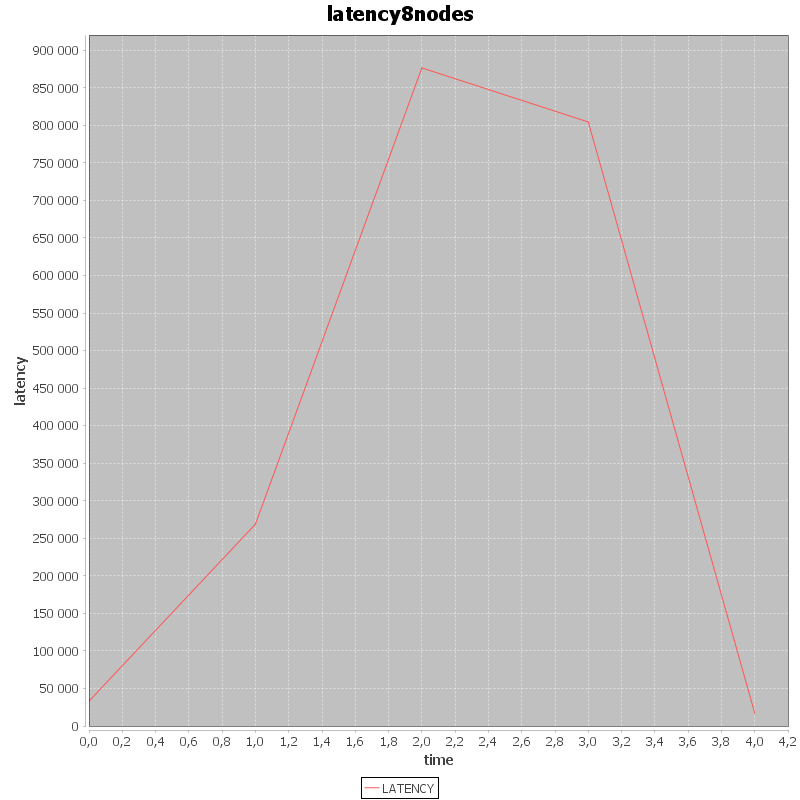
\includegraphics[scale=0.5]{latency8nodes.png}
\caption{Гистограма задержки по количеству сообщений}
 \label{figure:latency1}
\end{figure}

Можно заметить, что графики неравномерные. Это говорит о том, что сообщения передаются между узлами большими пачками. Например, на этом графике в первую в секунду обработалось 250 тыс. сообщений, а на второй уже 850 тысяч. 


Следующий интересный факт, замеченый мной: при увеличении количества узлов, количество обрабатываемых одним узлом сообщений падает. Это объясняется тем, что при количестве узлов больше, чем число потоков одновременно обрабатываемых системой, потоку банально не хватает времени для обработки одного сообщения.


\begin{figure}
\centering
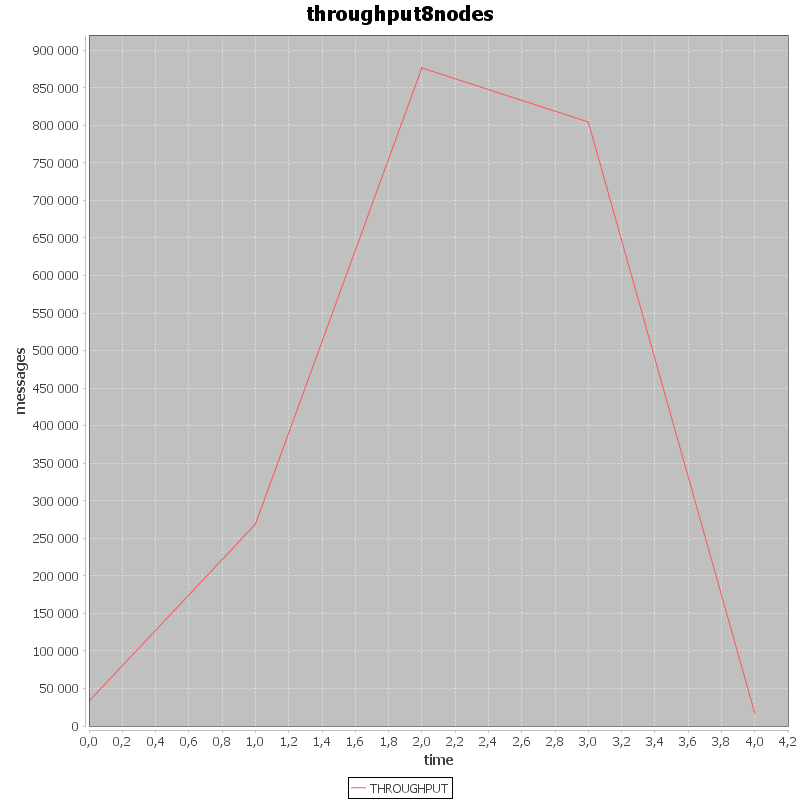
\includegraphics[scale=0.5]{throughput8nodes.png}
\caption{Пропускная способность системы в каждую единицу времени}
 \label{figure:throughput1}
\end{figure}

График пропускной способности подтверждает мои предлположения и делает их правдоподобными.

\chapter{Заключение}
Исследуя задачу, я пришёл к выводу, что не имеет смысла бесконечно увеличивать количество потоков. Оптимальное количество потоков в приложении - количество потоков, которое способна система/машина обрабатывать одновременно, т.е. зависит от процессора, ОС и остальных важных элементах системы. 

Стоить отметить ещё тот факт, что обратная ситуация тоже плохая: когда потоков, меньше, чем может \"позволить\" себе система, потокам выделяется слишком много времени, при котором они простаивают, либо слишком часто используют общую память так, что другие потоки не могут получить к ней доступ.

\end{document}


